\subsubsection{Iteratius}

La iteració és un recurs que s'empra en quasi tots els problemes de programació i es basa en una seqüència d'instruccions o codi que es repeteixen fins que s'arriba a un resultat final específic. \newline

Per iterar, en la majoria de llenguatges de programació, s'utilitzen bucles "for" o bucles "while". \newline

Un exemple molt típic de l'ús de la recursió i iteració és quan volem trobar el valor de la $n-esima$ posició de la seqüència de Fibonacci. \newline

La seqüència de Fibonacci és una seqüència infinita de nombres naturals, en la qual a partir del 0 i l'1, el valor dels següents nombres és la suma dels dos anteriors. \newline

Per entendre-ho millor, mirem la següent fórmula per calcular $F_n$, és a dir, per calcular qualsevol nombre de la seqüència de Fibonacci. \newline

F_n =
\begin{cases}
0 & \text{si $n = 0$}\\
1 & \text{si $n = 1$}\\
F_{n-1}+F_{n-2}& \text{si $n \geq 2$}
\end{cases} \newline \newline

Els primers nombres de la seqüència de Fibonacci són: [0, 1, 1, 2, 3, 5, 8, 13, 21, 34, 55...]

\begin{center}
    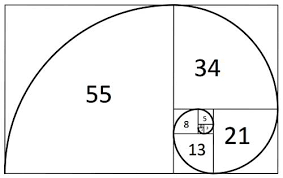
\includegraphics[width= .6 \textwidth]{fib.png}

    \caption{\emph{Figura 2: Seqüència de Fibonacci. Font: \url{https://www.brasilparalelo.com.br/artigos/o-que-e-fibonacci}}}
\end{center}

Donada qualsevol $n$ tal que la $n-esima$ posició en la seqüència de Fibonacci, amb l'ús de la iteració podem trobar $F_n$ amb una complexitat de $O(n)$.

\newpage

\begin{lstlisting}
int fib(int n){

    vector<int> F(n);
    // llista on guardem els valors de la seqüència

    F[0] = 0;
    F[1] = 1;

    for (int i = 2; i <= n; i++){ // iteració
        F[i] = F[i-1] + F[i-2];
        // f[i] és la suma dels dos anteriors nombres
    }
    return F[n];
}

int main(){
    int n; // Input -> 9
    cin >> n;
    cout << fib(n); // Output -> 34
}
\end{lstlisting}

Cal recalcar que inconscientment, en aquest algorisme iteratiu, estem fent un ús molt bàsic de la programació dinàmica (un algorisme del qual parlarem més endavant).

